\documentclass[12pt]{article}
\usepackage[
    marginparwidth=2.5cm, marginparsep=3mm
]{geometry}                % See geometry.pdf to learn the layout options. There are lots.
\geometry{letterpaper}                   % ... or a4paper or a5paper or ... 
%\geometry{landscape}                % Activate for for rotated page geometry
%\usepackage[parfill]{parskip}    % Activate to begin paragraphs with an empty line rather than an indent
\usepackage{float}
\usepackage{graphicx}
\graphicspath{{images/}}
\usepackage{amsmath,amssymb,amsfonts,amsthm}
\usepackage{epstopdf}
\usepackage{epigraph}
\usepackage{url}
\usepackage{mathtools}
\usepackage{tikz-cd}
\usepackage{hyperref}
%\usepackage{cleveref}
\usepackage[linewidth=0.2mm]{mdframed}
\usepackage{marginnote}
\renewcommand*{\marginfont}{\footnotesize}
\reversemarginpar

% Computer Concrete
%\usepackage{concmath}
%\usepackage[T1]{fontenc}

% Times variants
%
%\usepackage{mathptmx}
%\usepackage[T1]{fontenc}
%
%\usepackage[T1]{fontenc}
%\usepackage{stix}
%
% Needs to typeset using LuaLaTeX:
%\usepackage{unicode-math}
%\setmainfont{XITS}
%\setmathfont{XITS Math}

% garamond
%\usepackage[cmintegrals,cmbraces]{newtxmath}
%\usepackage{ebgaramond-maths}
%\usepackage[T1]{fontenc}


\DeclareGraphicsRule{.tif}{png}{.png}{`convert #1 `dirname #1`/`basename #1 .tif`.png}

\theoremstyle{plain}
\newtheorem{theorem}{Theorem}
\newtheorem{corollary}[theorem]{Corollary}
\newtheorem{lemma}[theorem]{Lemma}
\newtheorem{proposition}[theorem]{Proposition}
\newtheorem{conjecture}[theorem]{Conjecture}
\newtheorem{question}[theorem]{Question}
\newtheorem{definition}[theorem]{Definition}

\theoremstyle{definition}
\newtheorem{example}[theorem]{Example}
\newtheorem{todo}{TODO}

\theoremstyle{remark}
\newtheorem{remark}[theorem]{Remark}
\newtheorem{note}[theorem]{Note}
\newtheorem{intuition}[theorem]{Intuition}

\title{Physics}
\author{Nhan Trong}
\date{July 5, 2016---\today}                                           % Activate to display a given date or no date

\begin{document}
\sloppy
\maketitle

\epigraph{\textit{Everything should be made as simpa as possiba, but no simpla.}}{Albert Einstein}

\tableofcontents % remember to compile twice to update table of contents

\part{Electricity and Magnetism}

\begin{question}
Why do plastic and glass become negative and positively charged when rubbed with wool and silk?
\end{question}

\section{Insulators and Conductors}

\begin{note}
The third prong of the plug in electrical sockets connect to a wire that runs deep into the ground somewhere outside the building, thus grounding the appliance.
\end{note}

\begin{figure}[H]
\centering
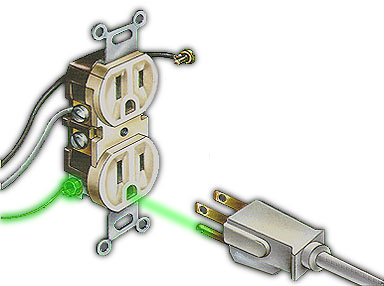
\includegraphics[width=.5\textwidth]{sg3p}
\end{figure}

\section{Some Special Field Configurations}

\begin{figure}[H]
\marginnote{Note that field lines usually don't describe the path of a charge moving in the field.}
\centering
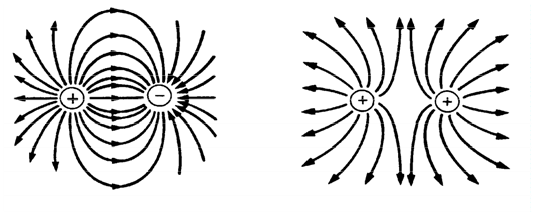
\includegraphics[width=1.0\textwidth]{201518-14415791-1040-instructionallab_manualsphysics6bexperiment_56b-exp4_fig2}
\caption{Electric Field}
\end{figure}

\subsection{Dipoles}

\subsubsection{Inverse Cube Law for Dipoles and Magnetic Fields}

\begin{mdframed}
\begin{proposition}[Inverse Cube Law for Dipoles]
The electric field of a dipole varies inversely as the distance cubed: $$F \propto \frac{Xx}{R^3}.$$
\end{proposition}
\end{mdframed}
\footnote{While researching Inverse Cube Law online I came across another unrelated but interesting law: the Square Cube Law due to Galileo: ``\textit{as a shape grows in size, its volume grows faster than its surface area. When applied to the real world this principle has many implications which are important in fields ranging from mechanical engineering to biomechanics. It helps explain phenomena including why large mammals like elephants have a harder time cooling themselves than small ones like mice, and why building taller and taller skyscrapers is increasingly difficult.}'' Hence this puts a limit on how big perfectly round land animals can be. You can be big, as long as you have complicated non-round shapes, like trees, or live in the water so it's easier to cool, like whales. (Of course there're other forces at work keeping an animal small, not just heating and cooling.)\\ \indent I wonder what the equivalent is in software engineering projects: the volume of code grows faster than the feature set, so that in order to make more features, you need to write more and more code? LOL Maybe this is why all software projects must end.}

\begin{proof}
\marginnote{What happens when they aren't?}
For simplicity assume the dipole and the test charge are aligned horizontally, so let the charge configuration be as follows:
\begin{figure}[H]
\centering
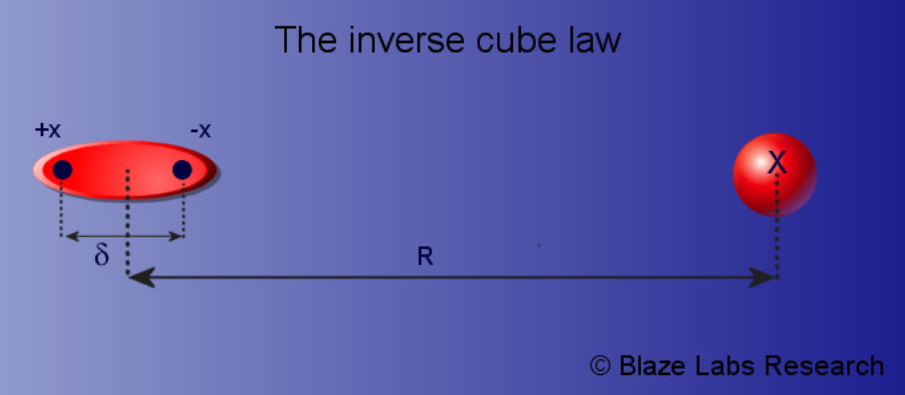
\includegraphics[width=0.7\textwidth]{inversecubedipole}
\end{figure}

Then the force acting on $X$ is $$F = \frac{KXx}{(R - \frac{\delta}{2})^2} - \frac{KXx}{(R + \frac{\delta}{2})^2} = \frac{KXx}{R^2(1 - \frac{\delta}{2R})^2} - \frac{KXx}{R^2(1 + \frac{\delta}{2R})^2}.$$
\marginnote{The Binomial Approximation is very useful and physicists use it a lot. I've seen it twice now.}To simplify this expression we'll use the Binomial Approximation, which says that if $x$ is a small number close to 0 and $\alpha$ is a real number, then $$(1 + x)^\alpha \approx 1 + \alpha x.$$
Applying this to the denominator, we get $$\left(1 \pm \frac{\delta}{2R}\right)^{-2} \approx 1 \mp \frac{\delta}{R}.$$

Now $F$ simplifies to $$F \approx \frac{KXx}{R^2}\left(1 + \frac{\delta}{R}\right) - \frac{KXx}{R^2}\left(1 - \frac{\delta}{R}\right) = \frac{2\delta KXx}{R^3}.\qedhere$$
\end{proof}

\begin{corollary}
Since magnets are always dipoles, magnetic fields also vary inversely as the distance cubed.
\end{corollary}

\begin{figure}[H]
\centering
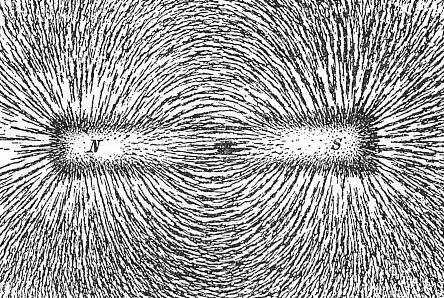
\includegraphics[width=.7\textwidth]{Magnet0873}
\end{figure}

\begin{example}[Atomic dipoles]
An atom in an electric field becomes a dipole since electrons will want to spend more time ``up stream'' than ``down stream''. (By convention an electric stream goes from positive to negative.)
\end{example}

\begin{figure}[H]
\centering
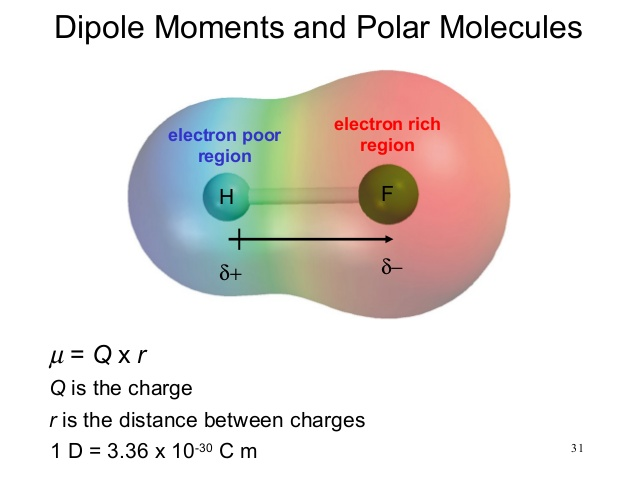
\includegraphics[width=.7\textwidth]{chapter-10-chemical-bonding-ii-molecular-geometry-and-hybridization-of-atomic-orbitals-31-638}
\end{figure}

\subsection{Infinite Uniformly Charged Plates}

\begin{proposition}
The electric field of an infinite uniformly charged plate is constant and equal to $$E = 2 \pi k \sigma = \frac{\sigma}{2 \epsilon},$$ where $\sigma$ is the charge density of the plate: the field is the same no matter where you are above the plate. Neat!
\end{proposition}

\begin{proof}
There are two ways to show this, using either Gauss's Law or direct integration. TODO.
\end{proof}

\centerline{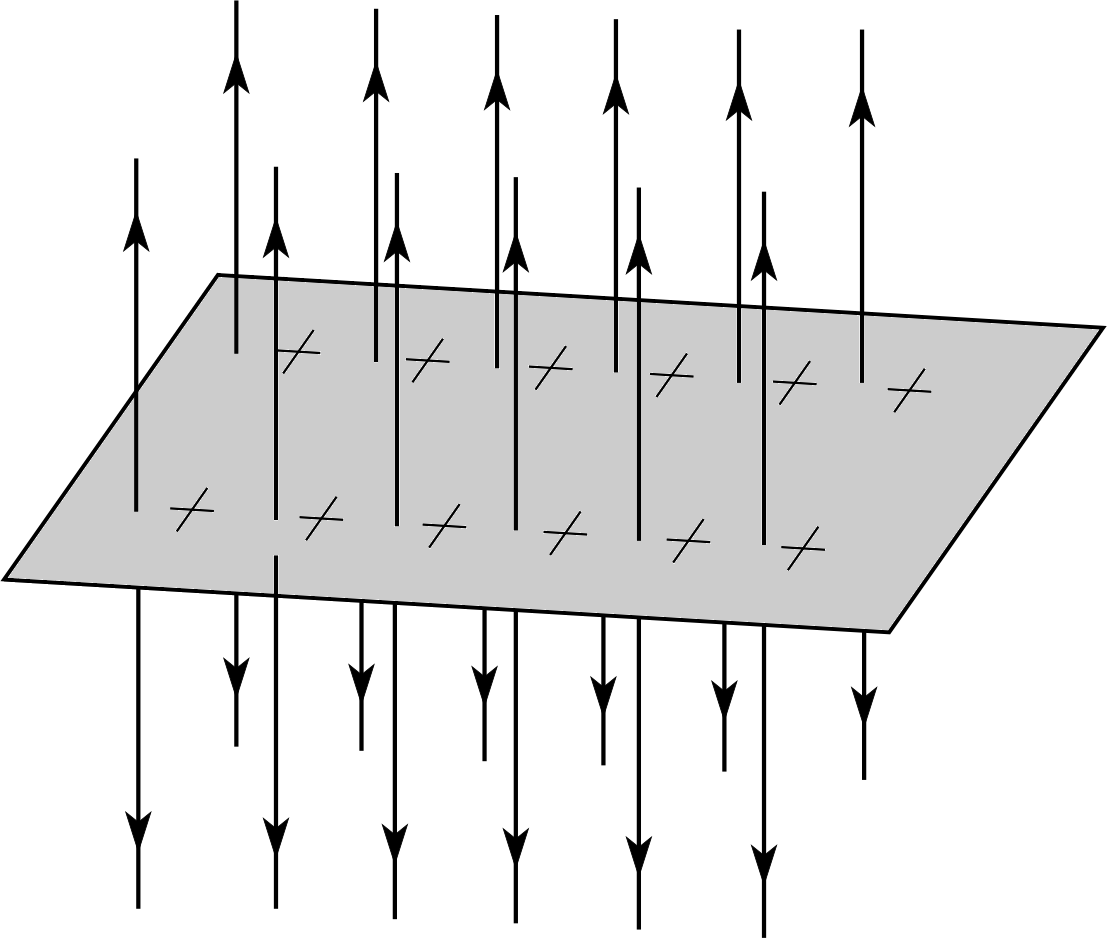
\includegraphics[width=.7\textwidth]{infiniteplate}}

\begin{corollary}
The electric field of an infinite uniformly charged plate with a hole at the origin is constant along the line above the origin.
\end{corollary}

\begin{question}
What does the rest of the field look like? Do the field lines converge towards the z-axis?
\end{question}

\begin{corollary}
If you had two parallel plates---instead of one---of opposite and equal charge densities, the electric field between the two plates would be twice as big: $$E = \pi k \sigma = \frac{\sigma}{\epsilon}.$$ Beyond those plates the field is zero because the plates cancel each other out.
\end{corollary}

\section*{Keywords}

Coulomb's Law, electric field, dipole, superposition, infinite uniformly charged plate, parallel plates, charge density, Gaussian surface, Gauss's Law / Flux Theorem, vacuum permittivity / electric constant, Coulomb's Constant, vacuum permeability / magnetic constant. Induction, Van de Graaff generator.

\begin{thebibliography}{99}

\bibitem{lewin} Walter Lewin's Physics Lectures.

\bibitem{} Images and everything else from the Internet.

\end{thebibliography}

\end{document}
